\let\negmedspace\undefined
\let\negthickspace\undefined
\documentclass[journal]{IEEEtran}
\usepackage[a4paper, margin=10mm, onecolumn]{geometry}
%\usepackage{lmodern} % Ensure lmodern is loaded for pdflatex
\usepackage{tfrupee} % Include tfrupee package

\setlength{\headheight}{1cm} % Set the height of the header box
\setlength{\headsep}{0mm}  % Set the distance between the header box and the top of the text

\usepackage{gvv-book}
\usepackage{gvv}
\usepackage{cite}
\usepackage{amsmath,amssymb,amsfonts,amsthm}
\usepackage{algorithmic}
\usepackage{graphicx}
\usepackage{float}
\usepackage{textcomp}
\usepackage{xcolor}
\usepackage{txfonts}
\usepackage{listings}
\usepackage{enumitem}
\usepackage{mathtools}
\usepackage{gensymb}
\usepackage{comment}
\usepackage[breaklinks=true]{hyperref}
\usepackage{tkz-euclide} 
\usepackage{listings}
% \usepackage{gvv}                                        
\def\inputGnumericTable{}                                 
\usepackage[latin1]{inputenc}                                
\usepackage{color}                                            
\usepackage{array}                                            
\usepackage{longtable}                                       
\usepackage{calc}                                             
\usepackage{multirow}                                         
\usepackage{hhline}                                           
\usepackage{ifthen}                                           
\usepackage{lscape}
\usepackage{tikz}
\usetikzlibrary{patterns}

\begin{document}

\bibliographystyle{IEEEtran}
\vspace{3cm}

\title{12.596}
\author{ee25btech11063-vejith}

\maketitle
% \maketitle
% \newpage
% \bigskip
{\let\newpage\relax\maketitle}
\renewcommand{\thefigure}{\theenumi}
\renewcommand{\thetable}{\theenumi}
\setlength{\intextsep}{10pt} % Space between text and floats
\textbf{Question}:\\
Consider the system of linear equations:\\
\hspace*{6cm} $x-2y+3z=-1$,\\
\hspace*{6cm} $x-3y+4z= 1$,\\
\hspace*{6cm} $-2x+4y-6z= k$\\
The value of $k$ for which the system has infinitely many solutions is \underline{\hspace{2cm}} \hspace{5cm} \brak{\text{EC } 2015}\\
\textbf{Solution}:\\
Given equations are
\begin{align}
    \brak{1 \hspace{0.3cm} -2 \hspace{0.4cm} 3}\myvec{x\\y\\z}=-1\\
     \brak{1 \hspace{0.3cm} -3 \hspace{0.4cm} 4}\myvec{x\\y\\z}=1\\
      \brak{-2 \hspace{0.3cm} 4 \hspace{0.4cm} -6}\myvec{x\\y\\z}=k
\end{align}
These equations can be written in matrix form as
\begin{align}
    \begin{pmatrix}
        1 & -2 & 3\\
        1 & -3 & 4\\
        -2 & 4 & -6
    \end{pmatrix}\myvec{x\\y\\z}=\myvec{-1\\1\\k}
\end{align}
Forming the augmented matrix
\begin{align}
    \left(\begin{array}{ccc|c}
        1 & -2 & 3 & -1 \\
        1 & -3 & 4 & 1\\
        -2 & 4 & -6 & k\\
\end{array}\right) &\xleftrightarrow{R_2 \leftarrow R_2 -  R_1} \left(\begin{array}{ccc|c}
        1 & -2 & 3 & -1 \\
        0 & -1 & 1 & 2\\
        -2 & 4 & -6 & k\\
\end{array}\right)\\
&\xleftrightarrow{R_3 \leftarrow R_3 +  2R_1} \left(\begin{array}{ccc|c}
        1 & -2 & 3 & -1 \\
        0 & -1 & 1 & 2\\
        0 & 0 & 0 & k-2\\
\end{array}\right)
\end{align}
As in the augmented matrix the entries of third  row are 0 their linear combination should also give 0 
\begin{align}
    k-2=0\\
    \implies k=2
\end{align}
Now the system has 2 equations and 3 variables which has infinite solutions
\begin{figure}[h!]
    \centering
    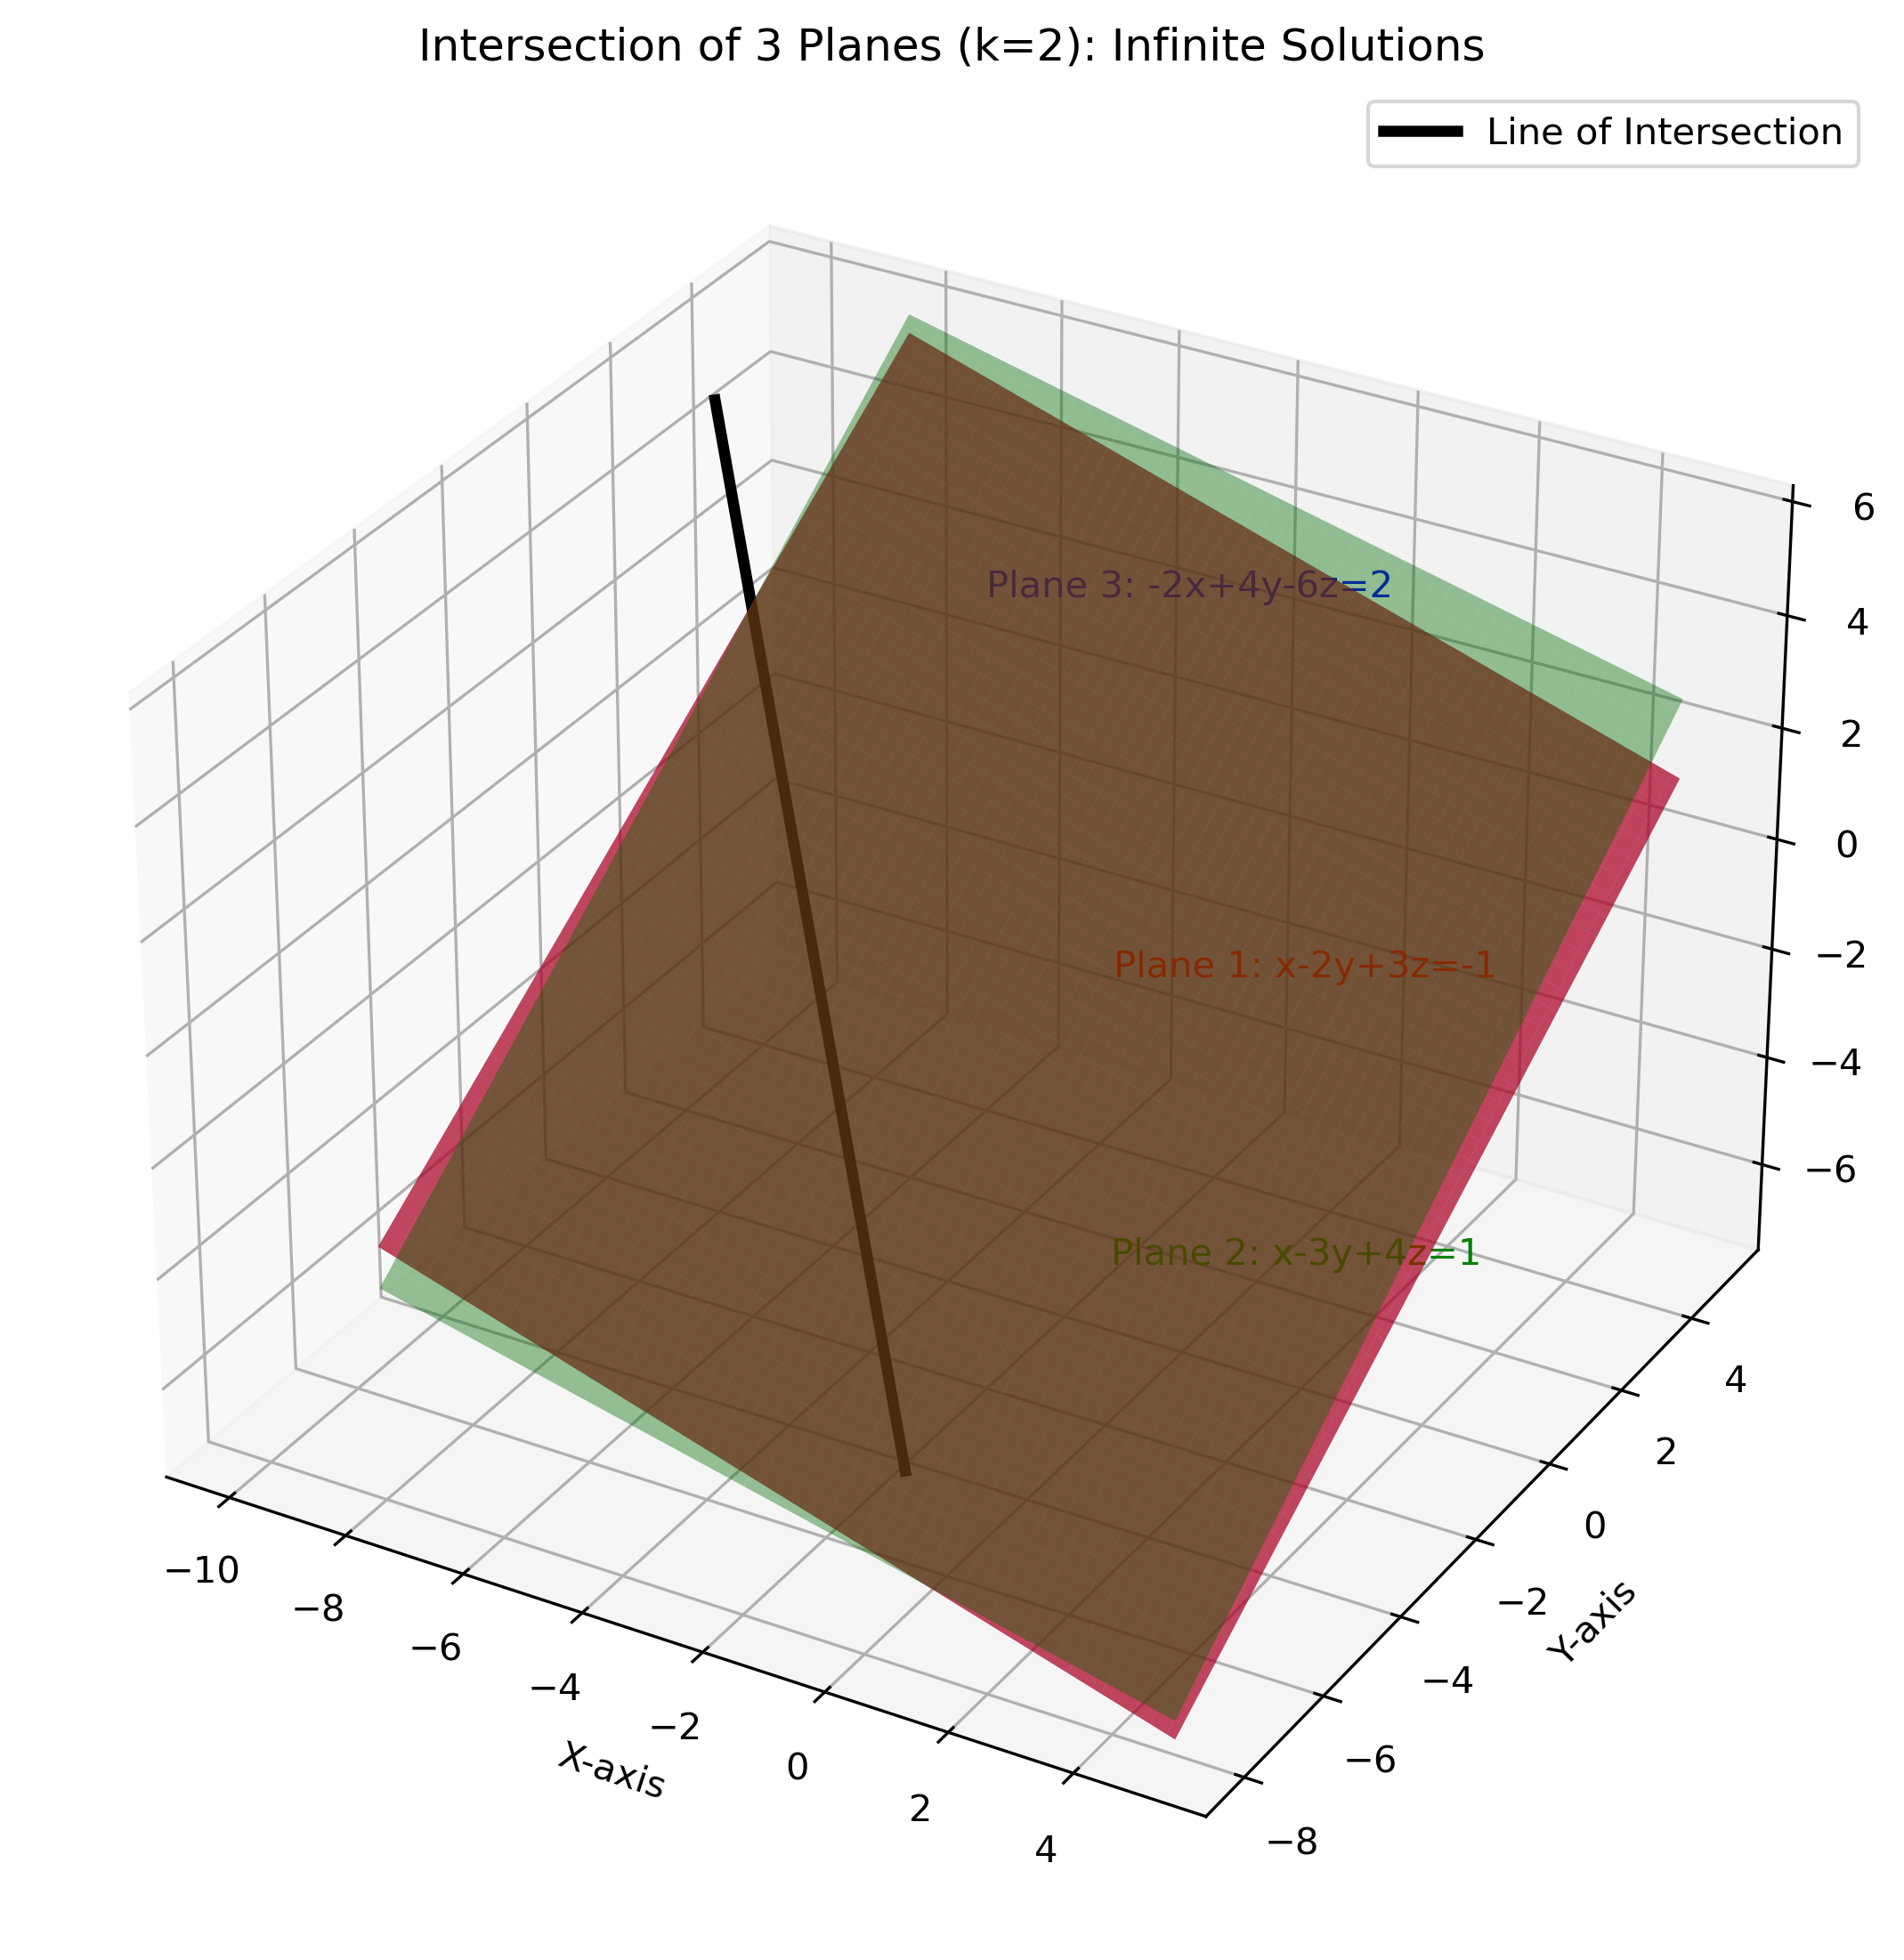
\includegraphics[width=0.74\columnwidth]{figs/01.png}
    \caption{}
    \label{fig:placeholder}
\end{figure}
\end{document}
